\documentclass[tikz,border=1pt]{standalone}
\usepackage{newtxtext}
\usepackage[scaled=0.92]{helvet}
\usetikzlibrary{positioning,arrows.meta,calc}
\definecolor{yel}{HTML}{F3E07A}
\definecolor{grn}{HTML}{8FDDA0}
\definecolor{pur}{HTML}{CDBCF4}
\definecolor{gry}{HTML}{E6E6E6}
\definecolor{shm}{HTML}{F7F7F7}
\definecolor{ink}{HTML}{222222}
\begin{document}
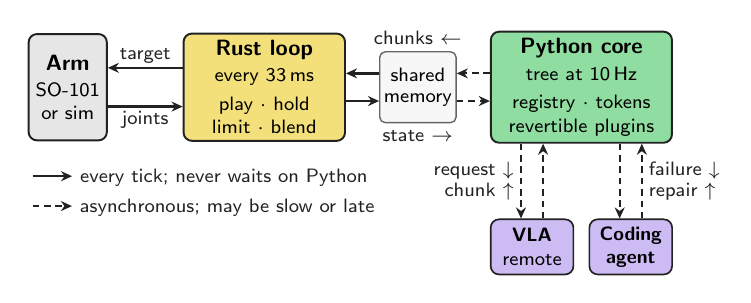
\begin{tikzpicture}[
  font=\sffamily\fontsize{7.2}{8.4}\selectfont,
  box/.style={rounded corners=3pt, draw=ink, line width=0.7pt, align=center, inner sep=2.5pt, minimum height=1.35cm},
  small/.style={rounded corners=3pt, draw=ink, line width=0.6pt, align=center, inner sep=2.5pt, minimum height=0.7cm, fill=pur},
  >={Stealth[length=4pt,width=3.6pt]},
  fast/.style={->, line width=0.85pt, ink},
  slow/.style={->, line width=0.75pt, ink, dash pattern=on 2.4pt off 1.7pt},
  lab/.style={font=\sffamily\fontsize{6.8}{7.8}\selectfont, inner sep=1.2pt, text=ink}
]
% ---------------------------------------------------------------- top row
\node[box, fill=gry, minimum width=0.95cm] (arm) {{\bfseries\fontsize{7.9}{9.2}\selectfont Arm}\\[1pt]SO-101\\or sim};
\node[box, fill=yel, minimum width=2.05cm, right=0.95cm of arm] (rust)
  {{\bfseries\fontsize{7.9}{9.2}\selectfont Rust loop}\\[1pt]every 33\,ms\\[2pt]play $\cdot$ hold\\limit $\cdot$ blend};
\node[rounded corners=2pt, draw=ink!70, line width=0.5pt, fill=shm, align=center, inner sep=1.5pt,
      minimum height=0.9cm, right=0.42cm of rust, font=\sffamily\fontsize{6.8}{7.8}\selectfont] (mem) {shared\\memory};
\node[box, fill=grn, minimum width=2.3cm, right=0.42cm of mem] (py)
  {{\bfseries\fontsize{7.9}{9.2}\selectfont Python core}\\[1pt]tree at 10\,Hz\\[2pt]registry $\cdot$ tokens\\revertible plugins};

% arm <-> rust (fast)
\draw[fast] ([yshift=7pt]rust.west) -- node[lab, above] {target} ([yshift=7pt]arm.east);
\draw[fast] ([yshift=-7pt]arm.east) -- node[lab, below] {joints} ([yshift=-7pt]rust.west);
% rust <-> memory (fast: read and written every tick)
\draw[fast] ([yshift=5pt]mem.west) -- ([yshift=5pt]rust.east);
\draw[fast] ([yshift=-5pt]rust.east) -- ([yshift=-5pt]mem.west);
% python <-> memory (slow: Python may stall)
\draw[slow] ([yshift=5pt]py.west) -- ([yshift=5pt]mem.east);
\draw[slow] ([yshift=-5pt]mem.east) -- ([yshift=-5pt]py.west);
\node[lab, above=1pt of mem] {chunks $\leftarrow$};
\node[lab, below=1pt of mem] {state $\rightarrow$};

% ---------------------------------------------------------------- slow row
\node[small, below=0.95cm of py.south west, anchor=north west, minimum width=1.05cm] (vla) {{\bfseries VLA}\\remote};
\node[small, below=0.95cm of py.south east, anchor=north east, minimum width=1.05cm] (agent) {{\bfseries Coding}\\{\bfseries agent}};
\draw[slow] ([xshift=-4pt]vla.north |- py.south) -- node[lab, left, align=right, xshift=-1pt] {request $\downarrow$\\chunk $\uparrow$} ([xshift=-4pt]vla.north);
\draw[slow] ([xshift=4pt]vla.north) -- ([xshift=4pt]vla.north |- py.south);
\draw[slow] ([xshift=-4pt]agent.north |- py.south) -- ([xshift=-4pt]agent.north);
\draw[slow] ([xshift=4pt]agent.north) -- node[lab, right, align=left, xshift=1pt] {failure $\downarrow$\\repair $\uparrow$} ([xshift=4pt]agent.north |- py.south);

% ---------------------------------------------------------------- legend
\node[lab, align=left, anchor=north west] at ([yshift=-0.30cm]arm.south west)
  {\tikz[baseline=-2.2pt]\draw[fast](0,0)--(0.5,0); every tick; never waits on Python\\[3pt]
   \tikz[baseline=-2.2pt]\draw[slow](0,0)--(0.5,0); asynchronous; may be slow or late};
\end{tikzpicture}
\end{document}
